\begin{isabellebody}\def\isabellecontext{Zipper}\isadelimtheory
\endisadelimtheory
\isatagtheory
\endisatagtheory
{\isafoldtheory}\isadelimtheory
\endisadelimtheory
\isamarkupsection{Zipper-based semantics of imperative programs\label{sec:source}}
\isamarkuptrue \isamarkupsubsection{The zipper data structure\label{sec:source_syntax}}
\isamarkuptrue \begin{isamarkuptext}Our plan is to propose an alternative technique to formalize operational 
semantics that will make it easier to preserve the execution context during
the translation to an automata-based formalism. Our technique is built around a zipper
data structure, whose purpose is to identify a location in a tree (in our
case: a \isa{stmt}) by the subtree below the location and the rest of the
tree (in our case: of type \isa{stmt{\isacharunderscore}path}).  In order to allow for an easy
navigation, the rest of the tree is turned inside-out so that it is possible
to reach the root of the tree by following the backwards pointers.
The following definition is a straightforward adaptation of the zipper for
binary trees discussed in \cite{Huet_zipper:1997} to the \isa{stmt} data
type:\end{isamarkuptext}\isamarkuptrue \isacommand{datatype}\isamarkupfalse \ stmt{\isacharunderscore}path\ {\isacharequal}\ \isanewline
\ \ PTop\isanewline
{\isacharbar}\ PSeqLeft\ stmt{\isacharunderscore}path\ stmt\ \ \ \ \ \ \ \ \ \ {\isacharbar}\ PSeqRight\ stmt\ stmt{\isacharunderscore}path\isanewline
{\isacharbar}\ PCondLeft\ expr\ stmt{\isacharunderscore}path\ stmt\ \ {\isacharbar}\ PCondRight\ expr\ stmt\ stmt{\isacharunderscore}path\isanewline
{\isacharbar}\ PWhile\ expr\ stmt{\isacharunderscore}path\begin{isamarkuptext}Here, \isa{PTop} represents the root of the original tree, and for
each constructor of \isa{stmt} and each of its sub-\isa{stmt}s, there is a
``hole'' of type \isa{stmt{\isacharunderscore}path} where a subtree can be fitted in. A
location in a tree is then a combination of a \isa{stmt} and a \isa{stmt{\isacharunderscore}path}:\end{isamarkuptext}\isamarkuptrue \isacommand{datatype}\isamarkupfalse \ stmt{\isacharunderscore}location\ {\isacharequal}\ Loc\ stmt\ stmt{\isacharunderscore}path\begin{isamarkuptext}Given a location in a tree, the function \isa{reconstruct} reconstructs the
 original tree \isa{reconstruct\ {\isacharcolon}{\isacharcolon}\ stmt\ {\isasymRightarrow}\ stmt{\isacharunderscore}path\ {\isasymRightarrow}\ stmt}, and \isa{reconstruct{\isacharunderscore}loc\ {\isacharparenleft}Loc\ c\ sp{\isacharparenright}\ {\isacharequal}\ reconstruct\ c\ sp} does the same for a location.\end{isamarkuptext}\isamarkuptrue \isacommand{fun}\isamarkupfalse \ reconstruct\ {\isacharcolon}{\isacharcolon}\ {\isachardoublequoteopen}stmt\ {\isasymRightarrow}\ stmt{\isacharunderscore}path\ {\isasymRightarrow}\ stmt{\isachardoublequoteclose}\ \isakeyword{where}\isanewline
\ \ {\isachardoublequoteopen}reconstruct\ c\ PTop\ {\isacharequal}\ c{\isachardoublequoteclose}\isanewline
{\isacharbar}\ {\isachardoublequoteopen}reconstruct\ c\ {\isacharparenleft}PSeqLeft\ sp\ c{\isadigit{2}}{\isacharparenright}\ {\isacharequal}\ reconstruct\ {\isacharparenleft}Seq\ c\ c{\isadigit{2}}{\isacharparenright}\ sp{\isachardoublequoteclose}\isanewline
{\isacharbar}\ {\isachardoublequoteopen}reconstruct\ c\ {\isacharparenleft}PSeqRight\ c{\isadigit{1}}\ sp{\isacharparenright}\ {\isacharequal}\ reconstruct\ {\isacharparenleft}Seq\ c{\isadigit{1}}\ c{\isacharparenright}\ sp{\isachardoublequoteclose}\isanewline
{\isacharbar}\ {\isachardoublequoteopen}reconstruct\ c\ {\isacharparenleft}PCondLeft\ e\ sp\ c{\isadigit{2}}{\isacharparenright}\ {\isacharequal}\ reconstruct\ {\isacharparenleft}Cond\ e\ c\ c{\isadigit{2}}{\isacharparenright}\ sp{\isachardoublequoteclose}\isanewline
{\isacharbar}\ {\isachardoublequoteopen}reconstruct\ c\ {\isacharparenleft}PCondRight\ e\ c{\isadigit{1}}\ sp{\isacharparenright}\ {\isacharequal}\ reconstruct\ {\isacharparenleft}Cond\ e\ c{\isadigit{1}}\ c{\isacharparenright}\ sp{\isachardoublequoteclose}\isanewline
{\isacharbar}\ {\isachardoublequoteopen}reconstruct\ c\ {\isacharparenleft}PWhile\ e\ sp{\isacharparenright}\ {\isacharequal}\ reconstruct\ {\isacharparenleft}While\ e\ c{\isacharparenright}\ sp{\isachardoublequoteclose}\isanewline
\isanewline
\isanewline
\isacommand{fun}\isamarkupfalse \ reconstruct{\isacharunderscore}loc\ {\isacharcolon}{\isacharcolon}\ {\isachardoublequoteopen}stmt{\isacharunderscore}location\ {\isasymRightarrow}\ stmt{\isachardoublequoteclose}\ \isakeyword{where}\isanewline
\ \ {\isachardoublequoteopen}reconstruct{\isacharunderscore}loc\ {\isacharparenleft}Loc\ c\ sp{\isacharparenright}\ {\isacharequal}\ reconstruct\ c\ sp{\isachardoublequoteclose}\isanewline
\isamarkupsubsection{Semantics\label{sec:source_sem}}
\isamarkuptrue \begin{isamarkuptext}Our semantics is a small-step operational semantics describing the
effect of the execution a program on a certain program state. For each
variable, the state yields \isa{Some} value associated with the variable, or
\isa{None} if the variable is unassigned. More formally, the state is a
mapping \isa{vname\ {\isasymRightarrow}\ val\ option}.  Defining the evaluation of an
expression in a state is then standard. 

Before commenting the rules of our semantics, let us discuss which kind
of structure we are manipulating. The semantics essentially consists in moving
around a pointer within the syntax tree. As explained in \secref{sec:source_syntax}, a
position in the syntax tree is given by a \isa{stmt{\isacharunderscore}location}. However,
during the traversal of the syntax tree, we visit each position at least twice
(and possibly several times, for example in a loop): before executing the
corresponding statement, and after finishing the execution. We therefore add a
Boolean flag, where \isa{True} is a marker for ``before'' and \isa{False}
for ``after'' execution. 

\begin{figure}

\hspace{-10ex}
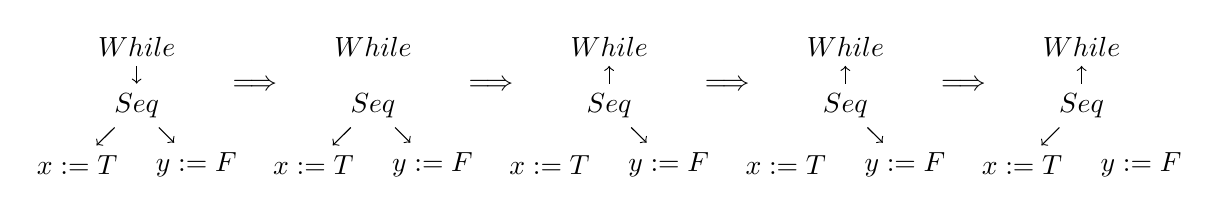
\begin{tikzpicture}[scale=0.5,level/.style={sibling distance = 20ex}]
\node at (0, 0) {$\beforeexec While$}
child {node {$Seq$}
  child {
    node {$x := T$}
    edge from parent [->]
  }
  child {
    node {$y := F$}
    edge from parent [->]
  }
  edge from parent [->]
};

\node at (3, -1) {$\Longrightarrow$};

\node at (6, 0) {$While$}
child {node {$\beforeexec Seq$}
  child {
    node {$x := T$}
    edge from parent [->]
  }
  child {
    node {$y := F$}
    edge from parent [->]
  }
  edge from parent [draw=none]  
};

\node at (9, -1) {$\Longrightarrow$};

\node at (12, 0) {$While$}
child {node {$Seq$}
  child {
    node {$\beforeexec x := T$}
    edge from parent [draw=none]
  }
  child {
    node {$y := F$}
    edge from parent [->]
  }
  edge from parent [<-]  
};

\node at (15, -1) {$\Longrightarrow$};

\node at (18, 0) {$While$}
child {node {$Seq$}
  child {
    node {$x := T\afterexec$}
    edge from parent [draw=none]
  }
  child {
    node {$y := F$}
    edge from parent [->]
  }
  edge from parent [<-]  
};

\node at (21, -1) {$\Longrightarrow$};

\node at (24, 0) {$While$}
child {node {$Seq$}
  child {
    node {$x := T$}
    edge from parent [->]
  }
  child {
    node {$\beforeexec y := F$}
    edge from parent [draw=none]
  }
  edge from parent [<-]  
};

\end{tikzpicture}


 \caption{Example of execution of small-step semantics}
\label{fig:example_execution_semantics}
\end{figure}

As an example, consider the execution sequence depicted in
\figref{fig:example_execution_semantics} (with assignments written in a more readable concrete syntax), consisting of the initial steps of
the execution of the program \isa{While\ {\isacharparenleft}e{\isacharcomma}\ Seq{\isacharparenleft}x\ {\isacharcolon}{\isacharequal}\ T{\isacharcomma}\ y\ {\isacharcolon}{\isacharequal}\ F{\isacharparenright}{\isacharparenright}}. The before
(resp.{} after) marker is indicated by a downward arrow before (resp.{} an upward
arrow behind) the current statement. 
The condition of the loop is omitted because it is irrelevant here. 
The middle configuration would be coded as
\isa{{\isacharparenleft}{\isacharparenleft}Loc\ {\isacharparenleft}x\ {\isacharcolon}{\isacharequal}\ T{\isacharparenright}\ {\isacharparenleft}PSeqLeft\ {\isacharparenleft}PWhile\ e\ PTop{\isacharparenright}\ {\isacharparenleft}y\ {\isacharcolon}{\isacharequal}\ F{\isacharparenright}{\isacharparenright}{\isacharparenright}{\isacharcomma}\ True{\isacharparenright}}.

Altogether, we obtain a syntactic configuration (\isa{synt{\isacharunderscore}config}) which
combines the location and the Boolean flag. The semantic configuration (\isa{sem{\isacharunderscore}config}) manipulated by the semantics adjoins the \isa{state}, as
defined previously.\end{isamarkuptext}\isamarkuptrue \isacommand{type{\isacharunderscore}synonym}\isamarkupfalse \ synt{\isacharunderscore}config\ {\isacharequal}\ {\isachardoublequoteopen}stmt{\isacharunderscore}location\ {\isasymtimes}\ bool{\isachardoublequoteclose}\isanewline
\isacommand{type{\isacharunderscore}synonym}\isamarkupfalse \ sem{\isacharunderscore}config\ {\isacharequal}\ {\isachardoublequoteopen}synt{\isacharunderscore}config\ {\isasymtimes}\ state{\isachardoublequoteclose}\begin{isamarkuptext}The rules of the small-step semantics of \figref{fig:smallStep} fall
into two categories: before execution of a statement \isa{s} (of the form \isa{{\isacharparenleft}{\isacharparenleft}l{\isacharcomma}\ True{\isacharparenright}{\isacharcomma}\ s{\isacharparenright}}) and after execution (of the form \isa{{\isacharparenleft}{\isacharparenleft}l{\isacharcomma}\ False{\isacharparenright}{\isacharcomma}\ s{\isacharparenright}});
there is only one rule of this latter kind: {\sc SFalse}.\end{isamarkuptext}\isamarkuptrue \begin{figure}[h!]
\isastyleminor\isamarkuptrue
\figline{}
\isacommand{fun}\isamarkupfalse \ next{\isacharunderscore}loc\ {\isacharcolon}{\isacharcolon}\ {\isachardoublequoteopen}stmt\ {\isasymRightarrow}\ stmt{\isacharunderscore}path\ {\isasymRightarrow}\ {\isacharparenleft}stmt{\isacharunderscore}location\ {\isasymtimes}\ bool{\isacharparenright}{\isachardoublequoteclose}\ \isakeyword{where}\isanewline
\ \ {\isachardoublequoteopen}next{\isacharunderscore}loc\ c\ PTop\ {\isacharequal}\ {\isacharparenleft}Loc\ c\ PTop{\isacharcomma}\ False{\isacharparenright}{\isachardoublequoteclose}\isanewline
{\isacharbar}\ {\isachardoublequoteopen}next{\isacharunderscore}loc\ c\ {\isacharparenleft}PSeqLeft\ sp\ c\isactrlsub {\isadigit{2}}{\isacharparenright}\ {\isacharequal}\ {\isacharparenleft}Loc\ c\isactrlsub {\isadigit{2}}\ {\isacharparenleft}PSeqRight\ c\ sp{\isacharparenright}{\isacharcomma}\ True{\isacharparenright}{\isachardoublequoteclose}\isanewline
{\isacharbar}\ {\isachardoublequoteopen}next{\isacharunderscore}loc\ c\ {\isacharparenleft}PSeqRight\ c\isactrlsub {\isadigit{1}}\ sp{\isacharparenright}\ {\isacharequal}\ {\isacharparenleft}Loc\ {\isacharparenleft}Seq\ \ c\isactrlsub {\isadigit{1}}\ c{\isacharparenright}\ sp{\isacharcomma}\ False{\isacharparenright}{\isachardoublequoteclose}\isanewline
{\isacharbar}\ {\isachardoublequoteopen}next{\isacharunderscore}loc\ c\ {\isacharparenleft}PCondLeft\ e\ sp\ c\isactrlsub {\isadigit{2}}{\isacharparenright}\ {\isacharequal}\ {\isacharparenleft}Loc\ {\isacharparenleft}Cond\ e\ c\ c\isactrlsub {\isadigit{2}}{\isacharparenright}\ sp{\isacharcomma}\ False{\isacharparenright}{\isachardoublequoteclose}\isanewline
{\isacharbar}\ {\isachardoublequoteopen}next{\isacharunderscore}loc\ c\ {\isacharparenleft}PCondRight\ e\ c\isactrlsub {\isadigit{1}}\ sp{\isacharparenright}\ {\isacharequal}\ {\isacharparenleft}Loc\ {\isacharparenleft}Cond\ e\ c\isactrlsub {\isadigit{1}}\ c{\isacharparenright}\ sp{\isacharcomma}\ False{\isacharparenright}{\isachardoublequoteclose}\isanewline
{\isacharbar}\ {\isachardoublequoteopen}next{\isacharunderscore}loc\ c\ {\isacharparenleft}PWhile\ e\ sp{\isacharparenright}\ {\isacharequal}\ {\isacharparenleft}Loc\ {\isacharparenleft}While\ e\ c{\isacharparenright}\ sp{\isacharcomma}\ True{\isacharparenright}{\isachardoublequoteclose}\newline
\figline{}
\caption{Finding the next location}\label{fig:next_loc}
\end{figure}
\isadelimproof
\endisadelimproof
\isatagproof
\endisatagproof
{\isafoldproof}\isadelimproof
\endisadelimproof
\begin{figure}[h!]
\isastyleminor\isamarkuptrue
\figline{}
\begin{isamarkuptext}\begin{center}
\begin{small}
\isa{\mbox{}\inferrule{\mbox{}}{\mbox{{\isacharparenleft}{\isacharparenleft}Loc\ Empty\ sp{\isacharcomma}\ True{\isacharparenright}{\isacharcomma}\ s{\isacharparenright}\ {\isasymrightarrow}\ {\isacharparenleft}{\isacharparenleft}Loc\ Empty\ sp{\isacharcomma}\ False{\isacharparenright}{\isacharcomma}\ s{\isacharparenright}}}}{\hspace{1ex} [\sc SEmpty]}\\[2ex]
\isa{\mbox{}\inferrule{\mbox{}}{\mbox{{\isacharparenleft}{\isacharparenleft}Loc\ {\isacharparenleft}Assign\ vr\ vl{\isacharparenright}\ sp{\isacharcomma}\ True{\isacharparenright}{\isacharcomma}\ s{\isacharparenright}\ {\isasymrightarrow}\ {\isacharparenleft}{\isacharparenleft}Loc\ {\isacharparenleft}Assign\ vr\ vl{\isacharparenright}\ sp{\isacharcomma}\ False{\isacharparenright}{\isacharcomma}\ s{\isacharparenleft}vr\ {\isasymmapsto}\ vl{\isacharparenright}{\isacharparenright}}}}{[\sc SAssign]}\\[2ex]
\isa{\mbox{}\inferrule{\mbox{}}{\mbox{{\isacharparenleft}{\isacharparenleft}Loc\ {\isacharparenleft}Seq\ c\isactrlsub {\isadigit{1}}\ c\isactrlsub {\isadigit{2}}{\isacharparenright}\ sp{\isacharcomma}\ True{\isacharparenright}{\isacharcomma}\ s{\isacharparenright}\ {\isasymrightarrow}\ {\isacharparenleft}{\isacharparenleft}Loc\ c\isactrlsub {\isadigit{1}}\ {\isacharparenleft}PSeqLeft\ sp\ c\isactrlsub {\isadigit{2}}{\isacharparenright}{\isacharcomma}\ True{\isacharparenright}{\isacharcomma}\ s{\isacharparenright}}}}{\hspace{1ex} [\sc SSeq]}\\[2ex]
\isa{\mbox{}\inferrule{\mbox{eval\ e\ s\ {\isacharequal}\ Bool\ True}}{\mbox{{\isacharparenleft}{\isacharparenleft}Loc\ {\isacharparenleft}Cond\ e\ c\isactrlsub {\isadigit{1}}\ c\isactrlsub {\isadigit{2}}{\isacharparenright}\ sp{\isacharcomma}\ True{\isacharparenright}{\isacharcomma}\ s{\isacharparenright}\ {\isasymrightarrow}\ {\isacharparenleft}{\isacharparenleft}Loc\ c\isactrlsub {\isadigit{1}}\ {\isacharparenleft}PCondLeft\ e\ sp\ c\isactrlsub {\isadigit{2}}{\isacharparenright}{\isacharcomma}\ True{\isacharparenright}{\isacharcomma}\ s{\isacharparenright}}}}{[\sc SCondT]}\\[2ex]
\isa{\mbox{}\inferrule{\mbox{eval\ e\ s\ {\isacharequal}\ Bool\ False}}{\mbox{{\isacharparenleft}{\isacharparenleft}Loc\ {\isacharparenleft}Cond\ e\ c\isactrlsub {\isadigit{1}}\ c\isactrlsub {\isadigit{2}}{\isacharparenright}\ sp{\isacharcomma}\ True{\isacharparenright}{\isacharcomma}\ s{\isacharparenright}\ {\isasymrightarrow}\ {\isacharparenleft}{\isacharparenleft}Loc\ c\isactrlsub {\isadigit{2}}\ {\isacharparenleft}PCondRight\ e\ c\isactrlsub {\isadigit{1}}\ sp{\isacharparenright}{\isacharcomma}\ True{\isacharparenright}{\isacharcomma}\ s{\isacharparenright}}}}{[\sc SCondF]}\\[2ex]
\isa{\mbox{}\inferrule{\mbox{eval\ e\ s\ {\isacharequal}\ Bool\ True}}{\mbox{{\isacharparenleft}{\isacharparenleft}Loc\ {\isacharparenleft}While\ e\ c{\isacharparenright}\ sp{\isacharcomma}\ True{\isacharparenright}{\isacharcomma}\ s{\isacharparenright}\ {\isasymrightarrow}\ {\isacharparenleft}{\isacharparenleft}Loc\ c\ {\isacharparenleft}PWhile\ e\ sp{\isacharparenright}{\isacharcomma}\ True{\isacharparenright}{\isacharcomma}\ s{\isacharparenright}}}}{\hspace{1ex} [\sc SWhileT]}\\[2ex]
\isa{\mbox{}\inferrule{\mbox{eval\ e\ s\ {\isacharequal}\ Bool\ False}}{\mbox{{\isacharparenleft}{\isacharparenleft}Loc\ {\isacharparenleft}While\ e\ c{\isacharparenright}\ sp{\isacharcomma}\ True{\isacharparenright}{\isacharcomma}\ s{\isacharparenright}\ {\isasymrightarrow}\ {\isacharparenleft}{\isacharparenleft}Loc\ {\isacharparenleft}While\ e\ c{\isacharparenright}\ sp{\isacharcomma}\ False{\isacharparenright}{\isacharcomma}\ s{\isacharparenright}}}}{\hspace{1ex} [\sc SWhileF]}\\[2ex]
\isa{\mbox{}\inferrule{\mbox{sp\ {\isasymnoteq}\ PTop}}{\mbox{{\isacharparenleft}{\isacharparenleft}Loc\ c\ sp{\isacharcomma}\ False{\isacharparenright}{\isacharcomma}\ s{\isacharparenright}\ {\isasymrightarrow}\ {\isacharparenleft}next{\isacharunderscore}loc\ c\ sp{\isacharcomma}\ s{\isacharparenright}}}}{\hspace{1ex} [\sc SFalse]}
\end{small}
\end{center}\end{isamarkuptext}\isamarkuptrue \figline{}
\caption{Small-step operational semantics}\label{fig:smallStep}
\end{figure}
\begin{isamarkuptext}Let us comment on the rules in detail:
\begin{itemize}
\item {\sc SEmpty} executes the \isa{Empty} statement just by swapping the Boolean flag.
\item {\sc SAssign} is similar, but it also updates the state for the assigned variable.
\item {\sc SSeq} moves the pointer to the substatement \isa{c\isactrlsub {\isadigit{1}}}, 
  pushing the substatement \isa{c\isactrlsub {\isadigit{2}}} as continuation to the statement path. 
\item {\sc SCondT} and {\sc SCondF} move to the \emph{then}- respectively \emph{else}- 
  branch of the conditional, depending on the value of the condition. 
\item {\sc SWhileT} moves to the body of the loop.
\item {\sc SWhileF} declares the execution of the loop as terminated, 
  by setting the Boolean flag to \isa{False}.
\item {\sc SFalse} comes into play when execution of the current statement is finished. 
  We then move to the next location, provided we have not already reached the root of 
  the syntax tree and the whole program terminates.
\end{itemize}

The move to the next relevant location is accomplished by function \isa{next{\isacharunderscore}loc} (\figref{fig:next_loc}) which intuitively works as follows: upon conclusion of the first substatement in
a sequence, we move to the second substatement. When finishing the body of a
loop, we move back to the beginning of the loop. In all other cases, we move
up the syntax tree, waiting for rule {\sc SFalse} to relaunch the
function.\end{isamarkuptext}\isamarkuptrue \isamarkupsection{Target language: Automata\label{sec:automata}}
\isamarkuptrue \isamarkupsubsection{Syntax\label{sec:automata_syntax}}
\isamarkuptrue \begin{isamarkuptext}As usual, our automata are a collection of nodes and edges,
with a distinguished initial state. In this general definition, we will keep the node type \isa{{\isacharprime}n} abstract. It will later be instantiated to \isa{synt{\isacharunderscore}config}.
An edge connects two nodes; moving along an edge may trigger an assignment to a
variable (\isa{AssAct}), or have no effect at all (\isa{NoAct}).

An automaton \isa{{\isacharprime}n\ ta} is a record consisting of a set of \isa{nodes}, a set of \isa{edges} and an initial node \isa{init{\isacharunderscore}s}. An edge has a \isa{source} node, an \isa{action} and a destination node \isa{dest}. Components of a record are written between \isa{{\isasymlparr}\ {\isachardot}{\isachardot}{\isachardot}\ {\isasymrparr}}.\end{isamarkuptext}\isamarkuptrue \isamarkupsubsection{Semantics\label{sec:automata_sem}}
\isamarkuptrue \begin{isamarkuptext}An automaton state is a node, together with a \isa{state} as in \secref{sec:source_sem}.\end{isamarkuptext}\isamarkuptrue \isacommand{type{\isacharunderscore}synonym}\isamarkupfalse \ {\isacharprime}n\ ta{\isacharunderscore}state\ {\isacharequal}\ {\isachardoublequoteopen}{\isacharprime}n\ {\isacharasterisk}\ state{\isachardoublequoteclose}\begin{isamarkuptext}Executing a step of an automaton in an automaton state \isa{{\isacharparenleft}l{\isacharcomma}\ s{\isacharparenright}} consists of selecting an edge starting in node \isa{l}, moving to the
target of the edge and executing its action. Automata are
non-deterministic; in this simplified model, we have no guards for selecting
edges.

\begin{center}
\isa{\mbox{}\inferrule{\mbox{e\ {\isasymin}\ set\ {\isacharparenleft}edges\ aut{\isacharparenright}}\\\ \mbox{l\ {\isacharequal}\ source\ e}\\\ \mbox{l{\isacharprime}\ {\isacharequal}\ dest\ e}\\\ \mbox{s{\isacharprime}\ {\isacharequal}\ action{\isacharunderscore}effect\ {\isacharparenleft}action\ e{\isacharparenright}\ s}}{\mbox{aut\ {\isasymturnstile}\ {\isacharparenleft}l{\isacharcomma}\ s{\isacharparenright}\ {\isasymrightarrow}\ {\isacharparenleft}l{\isacharprime}{\isacharcomma}\ s{\isacharprime}{\isacharparenright}\ }}}{\hspace{1ex} [\sc Action]}
\end{center}\end{isamarkuptext}\isamarkuptrue \isamarkupsection{Automata construction\label{sec:automata_construction}}
\isamarkuptrue \begin{isamarkuptext}The principle of abstracting a statement to an automaton is simple;
the novelty resides in the way the automaton is generated via the zipper
structure: as nodes, we choose the locations of the statements (with their
Boolean flags), and as edges all possible transitions of the semantics.

To make this precise, we need some auxiliary functions. We first define a
function \isa{all{\isacharunderscore}locations} of type \isa{stmt\ {\isasymRightarrow}\ stmt{\isacharunderscore}path\ {\isasymRightarrow}\ stmt{\isacharunderscore}location\ list} which gathers all locations in a statement, and a function \isa{nodes{\isacharunderscore}of{\isacharunderscore}stmt{\isacharunderscore}locations} which adds the Boolean flags.\end{isamarkuptext}\isamarkuptrue \begin{isamarkuptext}As for the edges, the function \isa{synt{\isacharunderscore}step{\isacharunderscore}image} yields all
possible successor configurations for a given syntactic configuration. This is of
course an over-approximation of the behavior of the semantics, since some of
the source tree locations may be unreachable during execution.\end{isamarkuptext}\isamarkuptrue \isacommand{fun}\isamarkupfalse \ synt{\isacharunderscore}step{\isacharunderscore}image\ {\isacharcolon}{\isacharcolon}\ {\isachardoublequoteopen}synt{\isacharunderscore}config\ {\isasymRightarrow}\ synt{\isacharunderscore}config\ list{\isachardoublequoteclose}\ \isakeyword{where}\isanewline
\ \ {\isachardoublequoteopen}synt{\isacharunderscore}step{\isacharunderscore}image\ {\isacharparenleft}Loc\ Empty\ sp{\isacharcomma}\ True{\isacharparenright}\ {\isacharequal}\ {\isacharbrackleft}{\isacharparenleft}Loc\ Empty\ sp{\isacharcomma}\ False{\isacharparenright}{\isacharbrackright}{\isachardoublequoteclose}\isanewline
{\isacharbar}\ {\isachardoublequoteopen}synt{\isacharunderscore}step{\isacharunderscore}image\ {\isacharparenleft}Loc\ {\isacharparenleft}Assign\ vr\ vl{\isacharparenright}\ sp{\isacharcomma}\ True{\isacharparenright}\ {\isacharequal}\ {\isacharbrackleft}{\isacharparenleft}Loc\ {\isacharparenleft}Assign\ vr\ vl{\isacharparenright}\ sp{\isacharcomma}\ False{\isacharparenright}{\isacharbrackright}{\isachardoublequoteclose}\isanewline
{\isacharbar}\ {\isachardoublequoteopen}synt{\isacharunderscore}step{\isacharunderscore}image\ {\isacharparenleft}Loc\ {\isacharparenleft}Seq\ c{\isadigit{1}}\ c{\isadigit{2}}{\isacharparenright}\ sp{\isacharcomma}\ True{\isacharparenright}\ {\isacharequal}\ {\isacharbrackleft}{\isacharparenleft}Loc\ c{\isadigit{1}}\ {\isacharparenleft}PSeqLeft\ sp\ c{\isadigit{2}}{\isacharparenright}{\isacharcomma}\ True{\isacharparenright}{\isacharbrackright}{\isachardoublequoteclose}\isanewline
{\isacharbar}\ {\isachardoublequoteopen}synt{\isacharunderscore}step{\isacharunderscore}image\ {\isacharparenleft}Loc\ {\isacharparenleft}Cond\ e\ c{\isadigit{1}}\ c{\isadigit{2}}{\isacharparenright}\ sp{\isacharcomma}\ True{\isacharparenright}\ {\isacharequal}\ \isanewline
\ \ \ \ \ \ \ \ \ \ \ \ \ \ {\isacharbrackleft}{\isacharparenleft}Loc\ c{\isadigit{1}}\ {\isacharparenleft}PCondLeft\ e\ sp\ c{\isadigit{2}}{\isacharparenright}{\isacharcomma}\ True{\isacharparenright}{\isacharcomma}\ {\isacharparenleft}Loc\ c{\isadigit{2}}\ {\isacharparenleft}PCondRight\ e\ c{\isadigit{1}}\ sp{\isacharparenright}{\isacharcomma}\ True{\isacharparenright}{\isacharbrackright}{\isachardoublequoteclose}\isanewline
{\isacharbar}\ {\isachardoublequoteopen}synt{\isacharunderscore}step{\isacharunderscore}image\ {\isacharparenleft}Loc\ {\isacharparenleft}While\ e\ c{\isacharparenright}\ sp{\isacharcomma}\ True{\isacharparenright}\ {\isacharequal}\ \isanewline
\ \ \ \ \ \ \ \ \ \ \ \ \ \ {\isacharbrackleft}{\isacharparenleft}Loc\ c\ {\isacharparenleft}PWhile\ e\ sp{\isacharparenright}{\isacharcomma}\ True{\isacharparenright}{\isacharcomma}\ {\isacharparenleft}Loc\ {\isacharparenleft}While\ e\ c{\isacharparenright}\ sp{\isacharcomma}\ False{\isacharparenright}{\isacharbrackright}{\isachardoublequoteclose}\isanewline
{\isacharbar}\ {\isachardoublequoteopen}synt{\isacharunderscore}step{\isacharunderscore}image\ {\isacharparenleft}Loc\ c\ sp{\isacharcomma}\ False{\isacharparenright}\ {\isacharequal}\ {\isacharparenleft}if\ sp\ {\isacharequal}\ PTop\ then\ {\isacharbrackleft}{\isacharbrackright}\ else\ {\isacharbrackleft}next{\isacharunderscore}loc\ c\ sp{\isacharbrackright}{\isacharparenright}{\isachardoublequoteclose}\begin{isamarkuptext}Together with the following definitions:\end{isamarkuptext}\isamarkuptrue \isacommand{fun}\isamarkupfalse \ action{\isacharunderscore}of{\isacharunderscore}synt{\isacharunderscore}config\ {\isacharcolon}{\isacharcolon}\ {\isachardoublequoteopen}synt{\isacharunderscore}config\ {\isasymRightarrow}\ action{\isachardoublequoteclose}\ \isakeyword{where}\isanewline
\ \ {\isachardoublequoteopen}action{\isacharunderscore}of{\isacharunderscore}synt{\isacharunderscore}config\ {\isacharparenleft}Loc\ {\isacharparenleft}Assign\ vn\ vl{\isacharparenright}\ sp{\isacharcomma}\ True{\isacharparenright}\ {\isacharequal}\ AssAct\ vn\ vl{\isachardoublequoteclose}\isanewline
{\isacharbar}\ {\isachardoublequoteopen}action{\isacharunderscore}of{\isacharunderscore}synt{\isacharunderscore}config\ {\isacharparenleft}Loc\ c\ sp{\isacharcomma}\ b{\isacharparenright}\ {\isacharequal}\ NoAct{\isachardoublequoteclose}\isanewline
\isanewline
\isacommand{definition}\isamarkupfalse \ edge{\isacharunderscore}of{\isacharunderscore}synt{\isacharunderscore}config\ {\isacharcolon}{\isacharcolon}\ {\isachardoublequoteopen}synt{\isacharunderscore}config\ {\isasymRightarrow}\ synt{\isacharunderscore}config\ edge\ list{\isachardoublequoteclose}\ \isakeyword{where}\isanewline
{\isachardoublequoteopen}edge{\isacharunderscore}of{\isacharunderscore}synt{\isacharunderscore}config\ s\ {\isacharequal}\ \isanewline
map{\isacharparenleft}{\isasymlambda}\ t{\isachardot}\ {\isasymlparr}source\ {\isacharequal}\ s{\isacharcomma}\ action\ {\isacharequal}\ action{\isacharunderscore}of{\isacharunderscore}synt{\isacharunderscore}config\ s{\isacharcomma}\ dest\ {\isacharequal}\ t{\isasymrparr}{\isacharparenright}{\isacharparenleft}synt{\isacharunderscore}step{\isacharunderscore}image\ s{\isacharparenright}{\isachardoublequoteclose}\isanewline
\isacommand{definition}\isamarkupfalse \ edges{\isacharunderscore}of{\isacharunderscore}nodes\ {\isacharcolon}{\isacharcolon}\ {\isachardoublequoteopen}synt{\isacharunderscore}config\ list\ {\isasymRightarrow}\ synt{\isacharunderscore}config\ edge\ list{\isachardoublequoteclose}\ \isakeyword{where}\isanewline
\ \ {\isachardoublequoteopen}edges{\isacharunderscore}of{\isacharunderscore}nodes\ nds\ {\isacharequal}\ concat\ {\isacharparenleft}map\ edge{\isacharunderscore}of{\isacharunderscore}synt{\isacharunderscore}config\ nds{\isacharparenright}{\isachardoublequoteclose}\begin{isamarkuptext}we can define the translation function from statements to automata:\end{isamarkuptext}\isamarkuptrue \isacommand{fun}\isamarkupfalse \ stmt{\isacharunderscore}to{\isacharunderscore}ta\ {\isacharcolon}{\isacharcolon}\ {\isachardoublequoteopen}stmt\ {\isasymRightarrow}\ synt{\isacharunderscore}config\ ta{\isachardoublequoteclose}\ \isakeyword{where}\isanewline
\ \ {\isachardoublequoteopen}stmt{\isacharunderscore}to{\isacharunderscore}ta\ c\ {\isacharequal}\ \isanewline
\ \ {\isacharparenleft}let\ nds\ {\isacharequal}\ nodes{\isacharunderscore}of{\isacharunderscore}stmt{\isacharunderscore}locations\ {\isacharparenleft}all{\isacharunderscore}locations\ c\ PTop{\isacharparenright}\ in\isanewline
\ \ \ {\isasymlparr}\ nodes\ {\isacharequal}\ nds{\isacharcomma}\ edges\ {\isacharequal}\ edges{\isacharunderscore}of{\isacharunderscore}nodes\ nds{\isacharcomma}\ init{\isacharunderscore}s\ {\isacharequal}\ {\isacharparenleft}{\isacharparenleft}Loc\ c\ PTop{\isacharparenright}{\isacharcomma}\ True{\isacharparenright}\ {\isasymrparr}{\isacharparenright}{\isachardoublequoteclose}\isanewline
\isadelimproof
\endisadelimproof
\isatagproof
\endisatagproof
{\isafoldproof}\isadelimproof
\endisadelimproof
\isadelimproof
\endisadelimproof
\isatagproof
\endisatagproof
{\isafoldproof}\isadelimproof
\endisadelimproof
\isadelimproof
\endisadelimproof
\isatagproof
\endisatagproof
{\isafoldproof}\isadelimproof
\endisadelimproof
\isadelimproof
\endisadelimproof
\isatagproof
\endisatagproof
{\isafoldproof}\isadelimproof
\endisadelimproof
\isadelimproof
\endisadelimproof
\isatagproof
\endisatagproof
{\isafoldproof}\isadelimproof
\endisadelimproof
\isadelimproof
\endisadelimproof
\isatagproof
\endisatagproof
{\isafoldproof}\isadelimproof
\endisadelimproof
\isadelimproof
\endisadelimproof
\isatagproof
\endisatagproof
{\isafoldproof}\isadelimproof
\endisadelimproof
\isadelimproof
\endisadelimproof
\isatagproof
\endisatagproof
{\isafoldproof}\isadelimproof
\endisadelimproof
\isadelimproof
\endisadelimproof
\isatagproof
\endisatagproof
{\isafoldproof}\isadelimproof
\endisadelimproof
\isadelimproof
\endisadelimproof
\isatagproof
\endisatagproof
{\isafoldproof}\isadelimproof
\endisadelimproof
\isadelimproof
\endisadelimproof
\isatagproof
\endisatagproof
{\isafoldproof}\isadelimproof
\endisadelimproof
\isamarkupsection{Simulation Property\label{sec:simulation_property}}
\isamarkuptrue \begin{isamarkuptext}We recall that the nodes of the automaton generated by \isa{stmt{\isacharunderscore}to{\isacharunderscore}ta} are labeled by configurations (location, Boolean flag) of the
syntax tree. The simulation lemma (\lemmaref{th:simulation_sem_aut}) holds for
automata with appropriate closure properties: a successor configuration wrt.{}
a transition of the semantics is also a label of the automaton (\isa{nodes{\isacharunderscore}closed}), and analogously for edges (\isa{edges{\isacharunderscore}closed}) or both nodes and edges 
(\isa{synt{\isacharunderscore}step{\isacharunderscore}image{\isacharunderscore}closed}).\end{isamarkuptext}\isamarkuptrue \isadelimproof
\endisadelimproof
\isatagproof
\endisatagproof
{\isafoldproof}\isadelimproof
\endisadelimproof
\begin{isamarkuptext}The simulation statement is a typical commuting-diagram property: a
step of the program semantics can be simulated by a step of the automaton
semantics, for corresponding program and automata states. For this
correspondence, we use the notation \isa{{\isasymapprox}}, even though it is just plain
syntactic equality in our case.
\begin{lemma}[Simulation property]\label{th:simulation_sem_aut}
\mbox{}\newline
Assume that \isa{synt{\isacharunderscore}step{\isacharunderscore}image{\isacharunderscore}closed\ aut} and \isa{{\isacharparenleft}{\isacharparenleft}{\isacharparenleft}lc{\isacharcomma}\ b{\isacharparenright}{\isacharcomma}\ s{\isacharparenright}\ {\isasymapprox}\ {\isacharparenleft}{\isacharparenleft}lca{\isacharcomma}\ ba{\isacharparenright}{\isacharcomma}\ sa{\isacharparenright}{\isacharparenright}}. If \isa{{\isacharparenleft}{\isacharparenleft}lc{\isacharcomma}\ b{\isacharparenright}{\isacharcomma}\ s{\isacharparenright}\ {\isasymrightarrow}\ {\isacharparenleft}{\isacharparenleft}lc{\isacharprime}{\isacharcomma}\ b{\isacharprime}{\isacharparenright}{\isacharcomma}\ s{\isacharprime}{\isacharparenright}}, then there exist \isa{lca{\isacharprime}{\isacharcomma}\ ba{\isacharprime}{\isacharcomma}\ sa{\isacharprime}} such that \isa{{\isacharparenleft}lca{\isacharprime}{\isacharcomma}\ ba{\isacharprime}{\isacharparenright}\ {\isasymin}\ set\ {\isacharparenleft}nodes\ aut{\isacharparenright}} and the automaton performs the same transition: \isa{aut\ {\isasymturnstile}\ {\isacharparenleft}{\isacharparenleft}lca{\isacharcomma}\ ba{\isacharparenright}{\isacharcomma}\ sa{\isacharparenright}\ {\isasymrightarrow}\ {\isacharparenleft}{\isacharparenleft}lca{\isacharprime}{\isacharcomma}\ ba{\isacharprime}{\isacharparenright}{\isacharcomma}\ sa{\isacharprime}{\isacharparenright}} and \isa{{\isacharparenleft}{\isacharparenleft}lc{\isacharprime}{\isacharcomma}\ b{\isacharprime}{\isacharparenright}{\isacharcomma}\ s{\isacharprime}{\isacharparenright}\ {\isasymapprox}\ {\isacharparenleft}{\isacharparenleft}lca{\isacharprime}{\isacharcomma}\ ba{\isacharprime}{\isacharparenright}{\isacharcomma}\ sa{\isacharprime}{\isacharparenright}}.
\end{lemma}
The proof is a simple induction over the transition relation of the program semantics and is almost fully automatic in the Isabelle proof assistant.\end{isamarkuptext}\isamarkuptrue \isadelimproof
\endisadelimproof
\isatagproof
\endisatagproof
{\isafoldproof}\isadelimproof
\endisadelimproof
\isadelimproof
\endisadelimproof
\isatagproof
\endisatagproof
{\isafoldproof}\isadelimproof
\endisadelimproof
\isadelimproof
\endisadelimproof
\isatagproof
\endisatagproof
{\isafoldproof}\isadelimproof
\endisadelimproof
\isadelimproof
\endisadelimproof
\isatagproof
\endisatagproof
{\isafoldproof}\isadelimproof
\endisadelimproof
\begin{isamarkuptext}We now want to get rid of the precondition \isa{synt{\isacharunderscore}step{\isacharunderscore}image{\isacharunderscore}closed\ aut} in
\lemmaref{th:simulation_sem_aut}. The first subcase (edge closure), is easy to prove. Node closure is  more difficult and requires the following key lemma:
\begin{lemma}\label{th:synt_step_image_all_locations}
\mbox{}\newline 
\isa{{\normalsize{}If\,}\ lc\ {\isasymin}\ set\ {\isacharparenleft}all{\isacharunderscore}locations\ c\ PTop{\isacharparenright}\ {\normalsize \,then\,}\ set\ {\isacharparenleft}map\ fst\ {\isacharparenleft}synt{\isacharunderscore}step{\isacharunderscore}image\ {\isacharparenleft}lc{\isacharcomma}\ b{\isacharparenright}{\isacharparenright}{\isacharparenright}\ {\isasymsubseteq}\ set\ {\isacharparenleft}all{\isacharunderscore}locations\ c\ PTop{\isacharparenright}{\isachardot}}
\end{lemma}
With this, we obtain the desired
\begin{lemma}[Closure of automaton]\label{th:synt_step_image_closed_stmt_to_ta}
\isa{synt{\isacharunderscore}step{\isacharunderscore}image{\isacharunderscore}closed\ {\isacharparenleft}stmt{\isacharunderscore}to{\isacharunderscore}ta\ c{\isacharparenright}}
\end{lemma}
For the proofs, see \cite{zipper_formalization}.\end{isamarkuptext}\isamarkuptrue \isadelimproof
\endisadelimproof
\isatagproof
\endisatagproof
{\isafoldproof}\isadelimproof
\endisadelimproof
\isadelimproof
\endisadelimproof
\isatagproof
\endisatagproof
{\isafoldproof}\isadelimproof
\endisadelimproof
\isadelimproof
\endisadelimproof
\isatagproof
\endisatagproof
{\isafoldproof}\isadelimproof
\endisadelimproof
\isadelimproof
\endisadelimproof
\isatagproof
\endisatagproof
{\isafoldproof}\isadelimproof
\endisadelimproof
\begin{isamarkuptext}Let us combine the previous results and write them
more succinctly, by using the notation \isa{{\isasymrightarrow}\isactrlsup {\isacharasterisk}} for the
reflexive-transitive closure for the transition relations of the small-step
semantics and the automaton. Whenever a state is reachable by executing a program \isa{c}
in its initial configuration, then a corresponding (\isa{{\isasymapprox}}) state is reachable 
by running the automaton generated with function \isa{stmt{\isacharunderscore}to{\isacharunderscore}ta}:

\begin{theorem}\label{th:simulation_generated}
\mbox{}\newline 
\isa{{\normalsize{}If\,}\ {\isacharparenleft}{\isacharparenleft}Loc\ c\ PTop{\isacharcomma}\ True{\isacharparenright}{\isacharcomma}\ s{\isacharparenright}\ {\isasymrightarrow}\isactrlsup {\isacharasterisk}\ {\isacharparenleft}cf{\isacharprime}{\isacharcomma}\ s{\isacharprime}{\isacharparenright}\ {\normalsize \,then\,}\ {\isasymexists}cfa{\isacharprime}\ sa{\isacharprime}{\isachardot}\ stmt{\isacharunderscore}to{\isacharunderscore}ta\ c\ {\isasymturnstile}\ {\isacharparenleft}init{\isacharunderscore}s\ {\isacharparenleft}stmt{\isacharunderscore}to{\isacharunderscore}ta\ c{\isacharparenright}{\isacharcomma}\ s{\isacharparenright}\ {\isasymrightarrow}\isactrlsup {\isacharasterisk}\ {\isacharparenleft}cfa{\isacharprime}{\isacharcomma}\ sa{\isacharprime}{\isacharparenright}\ \ {\isasymand}\ {\isacharparenleft}cf{\isacharprime}{\isacharcomma}\ s{\isacharprime}{\isacharparenright}\ {\isasymapprox}\ {\isacharparenleft}cfa{\isacharprime}{\isacharcomma}\ sa{\isacharprime}{\isacharparenright}{\isachardot}}
\end{theorem}

Obviously, the initial configuration of the semantics and the automaton are in
the simulation relation \isa{{\isasymapprox}}, and for the inductive step, we use
\lemmaref{th:simulation_sem_aut}.\end{isamarkuptext}\isamarkuptrue \isadelimtheory
\endisadelimtheory
\isatagtheory
\endisatagtheory
{\isafoldtheory}\isadelimtheory
\endisadelimtheory
\end{isabellebody}